\chapter{Model-based testing}
\section{Test generation}
Testing aims at showing that our system, which is under construction, is suited for our system requirements. With system testing we want to detect system failures and the differences between the expected output and the real implementation. 

Model-based testing is way to clarify these differences for our system under test (SUT). This test approach uses a model that encode the intended behaviour of the SUT and possibly the behaviour of its environment. This model should be simple, easy to understand according to the SUT complexity, and easy to check modify and maintain.
The idea of using test models is to avoid the unstructured tests written be hand. Consequently it must contains detailed information about the automatic generated tests. 

MBT is basically a matter of tooling so this impact the whole test process ,but not solves everything. Any change in the requirements or in the MBT model propagates to regenerate all the tests and review the correctness.

To fit the MBT into the developing process we must consider what inputs and outputs should be given.

Input artifacts:
\begin{itemize}
	\item Test strategy
	\item  The test basis including requirements and other test targets, test conditions, oral information, and 	existing design or models
	\item  Incident and defect reports, test logs and test execution logs from previous test execution activities
	\item  Method and process guidelines, tool documents
\end{itemize}
Output artifacts include different kinds of testware, such as:
\begin{itemize}
	\item  MBT models
	\item  Parts of the test plan (features to be tested, test environment, ...), test schedule, test metrics
	\item  Test scenarios, test suites, test execution schedules, test design specifications
	\item  Test cases, test procedure specifications, test data, test scripts, test adaptation layer (specifications and code)
	\item  Bidirectional traceability matrix between generated tests and the test basis, especially requirements, and defect reports
\end{itemize}

\section{General model-based testing process}

In this section I want to describe the general process of the model-based testing in 5 steps (\figref{mbtprocess}). 

\begin{figure}[!ht]
	\centering
	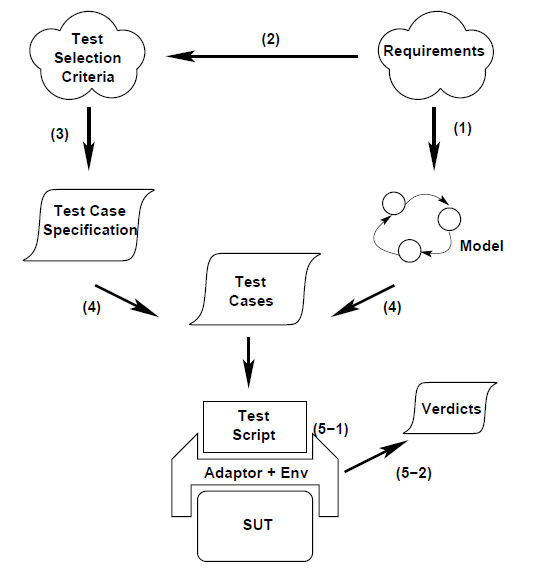
\includegraphics[width=100mm, keepaspectratio]{figures/MBTprocess.png}
	\caption{MBT process}
	\label{fig:mbtprocess}
\end{figure}

\textbf{Step 1.}
Our first task is to create a model of the SUT, which is implemented by considering the system requirements and specification documents. Our model could have an abstract level implementation, so we van forsake some functionality or certain quality-of-service attributes.

\textbf{Step 2}
In this step we define test selection criteria, which means that what is the goal of our tests. The best test is detect all system's failures and gives a helpful identifying what caused the failure. In general, test selection criteria can concentrate to functionality, structure of the model and well-defined set of faults.

\textbf{Step 3}
The previously defined selection criteria then transformed into test case specifications. This specification is a formal aspect of test selection criteria. 

\textbf{Step 4}
From the model and the test case specification are completed, a test suite is generated from them. Test case generators  pick randomly a test case, which satisfy a test case specification.

\textbf{Step 5-1}
Because of the abstraction of the model, each test case input and output concretisation handled by an abstraction layer called adaptor. The executing done by test script applying the considered input and output to the SUT and build the verdict. The adapter and the script is not entirely separated from each other.

\textbf{Step 5-2}
The adapter creates a verdict, which is the result of the comparsion. This can be \textit{pass}(if the expected and the actual output conform), \textit{fail} (if the expected does not match with the actual output) or \textit{inconclusive} (there is no decision yet).

\section{Model-based test generation dimensions}
\subsection{Subject of MBT models}
To create and effective and maintainable model avoid non-function aspects (like security, timing), further more consider the abstraction level of the model (who will discuss the test design). This can be a functional aspect (with limited functionality of the SUT), a data abstraction (expected input or/and output possibility restriction), a communication abstraction (mostly in protocol testing) and quality-of-service abstraction (like security, memory consumption).

Mainly three subjects can be reviewed for the model:
\textbf{System model}, which is describes the system with class or state diagrams.
\textbf{Environment model}, which can be deduced from the inputs and the usage of the SUT. This is an opposite aspect then the previous one.
\textbf{Test model}, which is a model of (one or several) test cases.

\subsection{Redundancy}
According to the SUT size, we can have multiple models for test suit. The models can have different aspect or different abstraction for more successful testing.

\subsection{Quality Characteristic}
Model quality directly affects the generated test output. MBT tools may check the syntax (model is consistent with the formal rules) and, at least partly, the semantic of the model (the content of the model is correct). Reviews check semantic and pragmatic quality (model is proper to test scenario and test generation)

\subsection{Test generation}
\subsubsection{Selection criteria}
From the same model various test suites can be generated. In this section test selection criteria will be described, which can help the tester to specify the right goal of the targeted tests. The coverage items may be \textbf{Requirements linked to MBT model} (full requirement sheet corresponds to the test cases), \textbf{MBT model elements} (Basically set coverage items to test cases like states, transition and decision in state diagrams). One more aspect is the \textbf{Data-related test selection criteria} which is related to test design techniques and may include heuristics such as pairwise test case generation.

\subsubsection{Technology}
This have the most biggest influence to the test generation results. This technology can be random path generation algorithm or search-based algorithms. In addition this technology could have more logic like model-checking (show a counterexample) and symbolic execution (to specific input, which part of the SUT executed) or deductive theorem proving (prove a statement).


\subsection{Test execution}

MBT generated test cases can be executed by manually or automatically. For manual execution the generated tests must be usable for manual test running. For automated test execution, test cases must be generated in a form that is executable. To test the SUT from abstract tests an adaptation layer code is needed to bridge the abstraction gap. This adaptation layer can be avoided by automated test scripts.

\subsection{On-line or Off-line test generation}
This approach is rather a technical detail of the test generation. With on-line generation, we can manipulate the SUT and test cases while executing them, which means parallel test case generation and execution. Consequently off-line generation is the idea that we create test cases before they are run.

\section{Model-based test generation tools}
What tools i have used, and what they are capable of.

\section{Graphwalker}

GraphWalker is an open source Model-based testing tool for test automation. It's designed to make it easy to create your tests using directed graphs. The tool generates test paths from these given graphs, which could be connected to each other. Each graph will have it's own set of generator(s) and stop condition(s).  An edge in the directed graph represent an action in the system, consequently a vertex means a verification state, where we can check assertions in code. A path is used to call the corresponding methods or functions of your SUT (system under test) by the adapter layer. 

The test selection is implemented by an expression, which have the following template: generator(stop\_condition\_type(condition))). This describes how to cover (random, a\_star, shortest\_all\_paths) and what to cover (edge\_coverage, vertex\_coverage, requirement\_coverage, dependency\_edge\_coverage, time\_duration, length, never).



There are two ways to generate tests by GraphWalker:
\begin{itemize}
	\item Offline: The path generation from the graph is done once (typically with command line), and these tests needs to be stored. A test automation system handle the tests. 
	\item Online: The path generation from the graph is created during the execution of the tests, run-time. If you have java coded SUT, it is pretty easy to add annotations to SUT and connect that to the generated paths. (command for Maven: \textit{mvn graphwalker:test})
\end{itemize}

For test execution an interface from the models is created by \textit{graphwalker:generate-sources} command. Our job is to implement these interfaces and call the proper SUT functionality for the given edges and vertexes.

\section{Pymodel}

The second Model-based test generation tool, which I have discovered is the Pymodel. This is an open-source framework implemented in Python. 

Basically it has 3 parts/programs
\begin{itemize}
	\item pma: PyModel analyzer: it's parameter gets models, which can b ea list os one or more modul names.  Each model contains a model (model program, FSM or test suite). This part generates FSM, the explored states and other result of the analysis.
	\item pmg: PyModel graphics: it's argument is an FSM (created by pma), and the program generates a file of commands in dot graph-drawing language (can be viewed by Graphviz). 
	\item pmt: PyModel tester: it's input parameter is a collection of models like in pma. The tester generates traces by executing the model. This programs offers several possibilities like view the traces, offline and online test generator execution (traces can be saved). 
\end{itemize}

The tool serves us one more program to invoke the 3 other parts with one single command, called pmv (PyModel viewer).
